\documentclass[runningheads,a4paper]{article}

\usepackage[utf8]{inputenc}

\setcounter{tocdepth}{3}

\usepackage[english]{babel} 
\usepackage{graphicx}
\usepackage{grffile}
\usepackage{float}
\usepackage{multicol}
\usepackage{url}
\usepackage{array}
\usepackage{wrapfig}
 \usepackage{multirow}
\usepackage{tabu}
\usepackage{amssymb}% http://ctan.org/pkg/amssymb
\usepackage{pifont}% http://ctan.org/pkg/pifont
\usepackage[font=small,labelfont=bf]{caption}

\newcommand{\cmark}{\ding{51}}%
\newcommand{\xmark}{\ding{55}}%

\usepackage{titling}
\usepackage[hidelinks]{hyperref}
\setcounter{secnumdepth}{5}
%Margins
\usepackage[
margin=2cm,
includefoot
]{geometry}


\graphicspath{{/}}

%Headers and Footers
\usepackage{fancyhdr}
\pagestyle{fancy}
\fancyhead{}
\fancyfoot{}
\fancyfoot[R]{\thepage}
\renewcommand{\headrulewidth}{0pt}
\renewcommand{\footrulewidth}{0pt}
\setlength\parindent{24pt}
\begin{document}
	
%Title Page
\begin{titlepage}
	\begin{center}
		
\includegraphics[width=10cm]{UP_Logo.PNG}  \\
		[1cm]
		\line(1,0){300} \\
		[0.3cm]
		\textsc{\Large
			Benchmarking Service\\
			Software Requirements Specification\\
			\hfill
			%University of Pretoria
		}\\
		[0.1cm]
		\line(1,0){300} \\
		[0.7cm]
		\textsc{\Large
			ProCoders
		} \\
	\end{center}
	
	\begin{center}
		\begin{centre}
			\textsc{\large\\
				Bongani Tshela - 14134790\\ 
			}
		
				\textsc{\large\\
					Harris Leshaba - 15312144\\ 
				}
			\textsc{\large\\
				Joseph Letsoalo - 15043844\\ 
			}
			
			\textsc{\large\\
				Minal Pramlall - 13288157\\ 
			}
			

            

		\end{centre}
		
		
		
	\end{center}
\end{titlepage}
%\maketitle%%%%%%%%%%%%%%%%%%%%%%%%%%%%%%%%%%%%%%%%%%%%%%%%%%%%%%%%%%%%%%%%%%%%

\begingroup

\tableofcontents
\addcontentsline{toc}{section}{Table Of Contents}
\endgroup
\newpage
\section{Project Scope}
The core of the system is a benchmarking tool which. The high level modules and their responsibilities are
shown in Figure 1
\section{User management module}
\subsection{Scope}
The scope of the user management module is shown in Figure 1. The user
management module is responsible for maintaining information about the registered
users of the system, including the authority levels of each user. User can manage their benchmarking records like deleting and storing new records, view them and retrieving old algorithm they have stored.

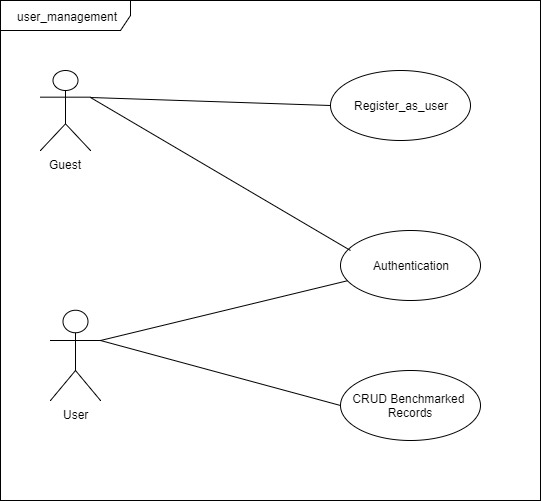
\includegraphics[width=7cm,height=10cm]{userDiagram.jpg}
\newline 
\textit{Figure 1} use case.
\newline
\newline No information is stored for the guest user. When accessing the service, the user
assumes the guest role without being logged in. The guest user may use public
services and my register or log in.
When a user is registered, the fields shown in the domain model are stored for the
user using a unique automatically assigned ID. The user provides all other fields. The
password is stored in encrypted format. The user can access all the services provided by the service
The register as user  use case is initiated by an end-user to create an account.\newline\newline
A user will not be created if the email specified in the request to create a user is already
associated with an existing user. This is done to ensure that if a user is already associated
with the email address, the user is given access to his/her profile instead of creating a new
user.\newline\newline
Note that this use case will use the \textbf{getUser(userEmail)} service provided by the module to
confirm if another user with that same email already exists in the system. A user should
only be created if \textbf{getUser(userEmail)} throws the \textit{noSuchUser} exception.
After the account has been created a notification will be sent to the user. The system have two types of users: Guest user and Registered user.
\subsubsection{\textbf{Domain model}}
The users management domain model is shown in Figure 2
\newline
\newline
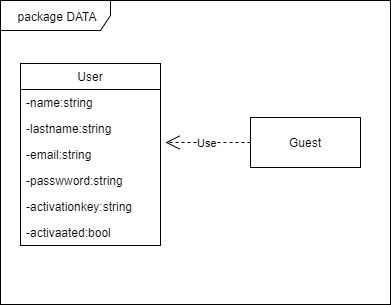
\includegraphics[width=7cm,height=8cm]{userClass.jpg}
\newline 
\textit{Figure 2} class diagram.

\subsubsection{\textbf{Precondition Table}}
CU1 \textbf{getUserEmail(email)}
\newline
\newline
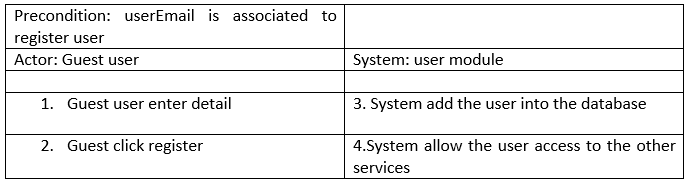
\includegraphics[width=12cm,height=3cm]{preUser.PNG}
\newline 
\textit{Figure 3} class diagram.

\subsection{\textbf{Service contracts}}
The following services should be provided
\newline
\newline
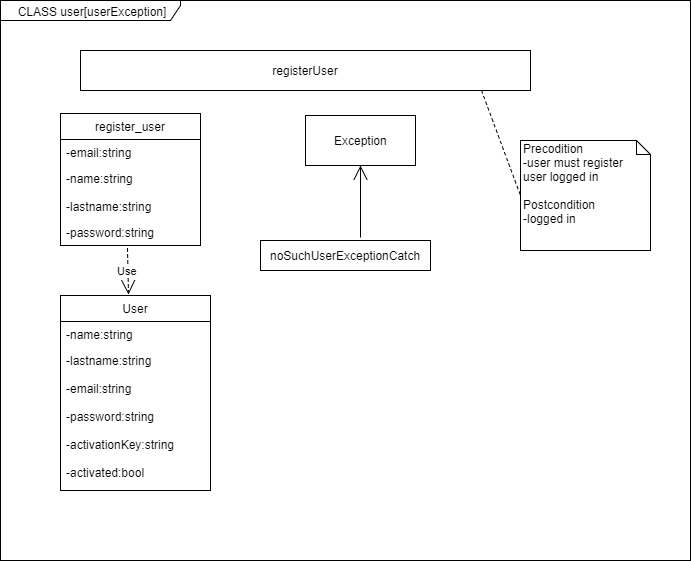
\includegraphics[width=12cm,height=10cm]{userConstract.jpg}
\newline 
\textit{Figure 4} class diagram.

\end{document}

